\documentclass[12pt,1in]{article}
\usepackage{amsmath, amssymb}
\usepackage{physics}
\usepackage[margin=1in]{geometry}
\usepackage{cite}
\usepackage{booktabs}
\usepackage{graphicx}
\usepackage{epstopdf}
\usepackage{float}
\newenvironment{Example}[2][Example]{\begin{trivlist}
		\item[\hskip \labelsep {\bfseries #1}\hskip \labelsep {\bfseries #2.}]}{\end{trivlist}}
\usepackage{hyperref}

\title{Analyzing Non-linear Ordinary Differential Equations\\ {\small MATH 26600}}
\author{Rutuj Gavankar}
\date{}
\begin{document}

\maketitle

\section{Introduction}

\subsection{Linearizing a system}


Let 
\begin{align}
\derivative{x}{t} &= F(x, y) \\
\derivative{y}{t} &= G(x , y)
\end{align}
be a system of first-order differential equations. The steady-state solutions of this system are the solutions for which  $x(t)$ and $y(t)$ are invariant. That is to say,
\begin{align}
    F(x,y) &= 0 \\
    G(x,y) &= 0
\end{align}
We can analyzing this system around these equilibrium points by making linear approximations of the function around these points. Using first order Taylor series expansion for $F$ and $G$ we get
\begin{align}
    F(x,y) &\approx F(x_0, y_0) + F_x(x_0, y_0)(x - x_0) + F_y(x_0, y_0)(y - y_0) \\
    G(x,y) &\approx G(x_0, y_0) + G_x(x_0, y_0)(x - x_0) + G_y(x_0, y_0)(y - y_0)
\end{align}
Where $x_0$ and $y_0$ are the equilibrium points for the system. The system can be re-written in matrix-vector notation as 
\begin{align}
    \begin{bmatrix}
    \derivative{x}{t} \\
    \derivative{y}{t}
    \end{bmatrix} &= 
    \begin{bmatrix}
    F_x(x_0, y_0) & F_y(x_0, y_0)\\
    G_x(x_0, y_0) & G_y(x_0, y_0)
    \end{bmatrix}
    \begin{bmatrix}
    x - x_0 \\
    y - y_0
    \end{bmatrix}
\end{align}Now, let $x - x_0$ be $u$ and $y - y_0$ be $v$, and $\Vec{v}$ be the vector $\left<u ,v\right>$
\begin{align}
    \therefore \derivative{\Vec{v}}{t} &= J\Vec{v} \label{eq:vec_mat}
\end{align}
Where $J$ is the Jacobian matrix, $$J = \begin{bmatrix}
    F_x(x_0, y_0) & F_y(x_0, y_0)\\
    G_x(x_0, y_0) & G_y(x_0, y_0)
    \end{bmatrix}$$
Now, Eq. \ref{eq:vec_mat} is an eigenvalue problem. The local stability and the behaviour of the system around the equilibrium points can be inferred from the eigenvalues of $J$. 

\subsection{Characterizing a system}
Near the equilibrium points, the non-linear system has similar behavior to the linear approximation, and thus, the stability of the system can be analyzed by analyzing the eigenvalues of the system. Let $\lambda_{1,2}$ be the eigenvalues of the system.
\begin{enumerate}
	\item If the eigenvalues of the system are real and positive at an equilibrium point, ($\lambda_{1,2} > 0$), the point is a \emph{nodal-source}. The solutions tend to diverge away from this point. The system is unstable around this point. 
	\item If the eigenvalues of the system are real and negative at an equilibrium point, ($\lambda_{1,2} < 0$),the point is a \emph{nodal-sink}. The solutions tend to converge towards this point. The system is stable around this point. 
	\item If the eigenvalues of the system are real, but $\lambda_1 < 0$ and $\lambda_2 > 0$, the point is a saddle point. The solutions tend to diverge away from this point. The system is unstable around this point.
	\item If the eigenvalues of the system imaginary, $(\lambda_{1,2} = \pm k i)$, the point is a \emph{center}.  The solutions tend to oscillate around this point. The system is stable around this point.
	\item If the eigenvalues of the system are complex, $(\lambda_{1,2} = a \pm b i)$, and $\Re{\lambda_{1,2}}> 0$, the point is a \emph{spiral-source}. The solutions tend to 
\end{enumerate}

\subsection{Quantitative Analysis of a System}

\subsection{Examples and Solutions}
\begin{Example}{1} \cite[p.~488]{diff_eq}
	Consider the system for $(x,y \geq 0)$
	\begin{align*}
    \derivative{x}{t} &= x(10 - x - y) \\
    \derivative{y}{t} &= y(30 - 2x - y)
\end{align*}
The Jacobian of the system is 
\begin{align*}
    J = \begin{bmatrix}
    10 - 2x - y & -x \\
    -2y & 30 - 2x - 2y
    \end{bmatrix}
\end{align*}
The system has equilibrium points at $(0,0)$, $(10,0)$, $(0,30)$. Analyzing the system at $(0,0)$,
\begin{align*}
    J|_{(0,0)} &= \begin{bmatrix}
    10 & 0 \\
    0 & 30
    \end{bmatrix}
\end{align*}
Since $J$ is a diagonal matrix, the eigenvalues of $J$ are the elements along its diagonal. That is, $\lambda_{1,2} = \{ 10, 30 \}$. Since both the eigenvalues are real and positive, the point $(0,0)$ is a nodal-source.
Similarly, analyzing the system at $(10,0)$,
\begin{align*}
    J|_{(10,0)} &= 
    \begin{bmatrix}
    -10 & -10\\
    0 & 10 
    \end{bmatrix}
\end{align*}
The eigenvalues of $J$ are $\lambda_{1,2} = \{-10, 10\}$. Since both the eigenvalues are real and nonzero, and $\lambda_1 < 0$, $\lambda_2 > 0$, the point $(10,0)$ is a saddle point. 
Now analyzing the system at $(0,30)$,
\begin{align*}
J|_{(0,30)} &= \begin{bmatrix}
-20 & 0 \\
-60 & -30 
\end{bmatrix}
\end{align*}
The eigenvalues for $J$ are $\lambda_{1,2} = \{-30, -20\}$. Since both eigenvalues are real and negative, $(0,30)$ is a nodal-sink. 
Now to graphically analyze the system, the nullclines can be plotted in the phase plane.
To find the horizontal nullclines,
\begin{align*}
\derivative{x}{t} &= 0\\
\therefore x(10 - x -y) &= 0
\end{align*}
That is, $x = 0$ or $y = 10 - x$. 
To find the vertical nullclines,
\begin{align*}
\derivative{y}{t} &= 0\\
\therefore y(30 - 2x - y) &= 0
\end{align*}
That is, $y = 0$ or $y = 30 - 2x$. 
\end{Example}

\begin{Example}{2}
	\cite[p.~488]{diff_eq}
	Consider the system for $(x,y \geq 0)$
	\begin{align*}
	\derivative{x}{t} &= x(2 - x - y)\\
	\derivative{y}{t} &= y(y - x^2)
	\end{align*}
	The Jacobian of the system is
	\begin{align*}
	J = \begin{bmatrix}
	2 -2x  -y & -x \\
	-2xy & 2y - x^2 
	\end{bmatrix}
	\end{align*}
	Steady-states in the region $(x,y \geq 0)$ are $(0,0)$ , $(1,1)$ and $(2,0)$. Analyzing point $(0,0)$,
	\begin{align*}
	J = \begin{bmatrix}
	2 & 0 \\
	0 & 0
	\end{bmatrix}
	\end{align*}
	The eigenvalues of $J$ are $\lambda_{1,2} = \{2, 0\}$
	
	
\begin{figure}[H]
	\centering
	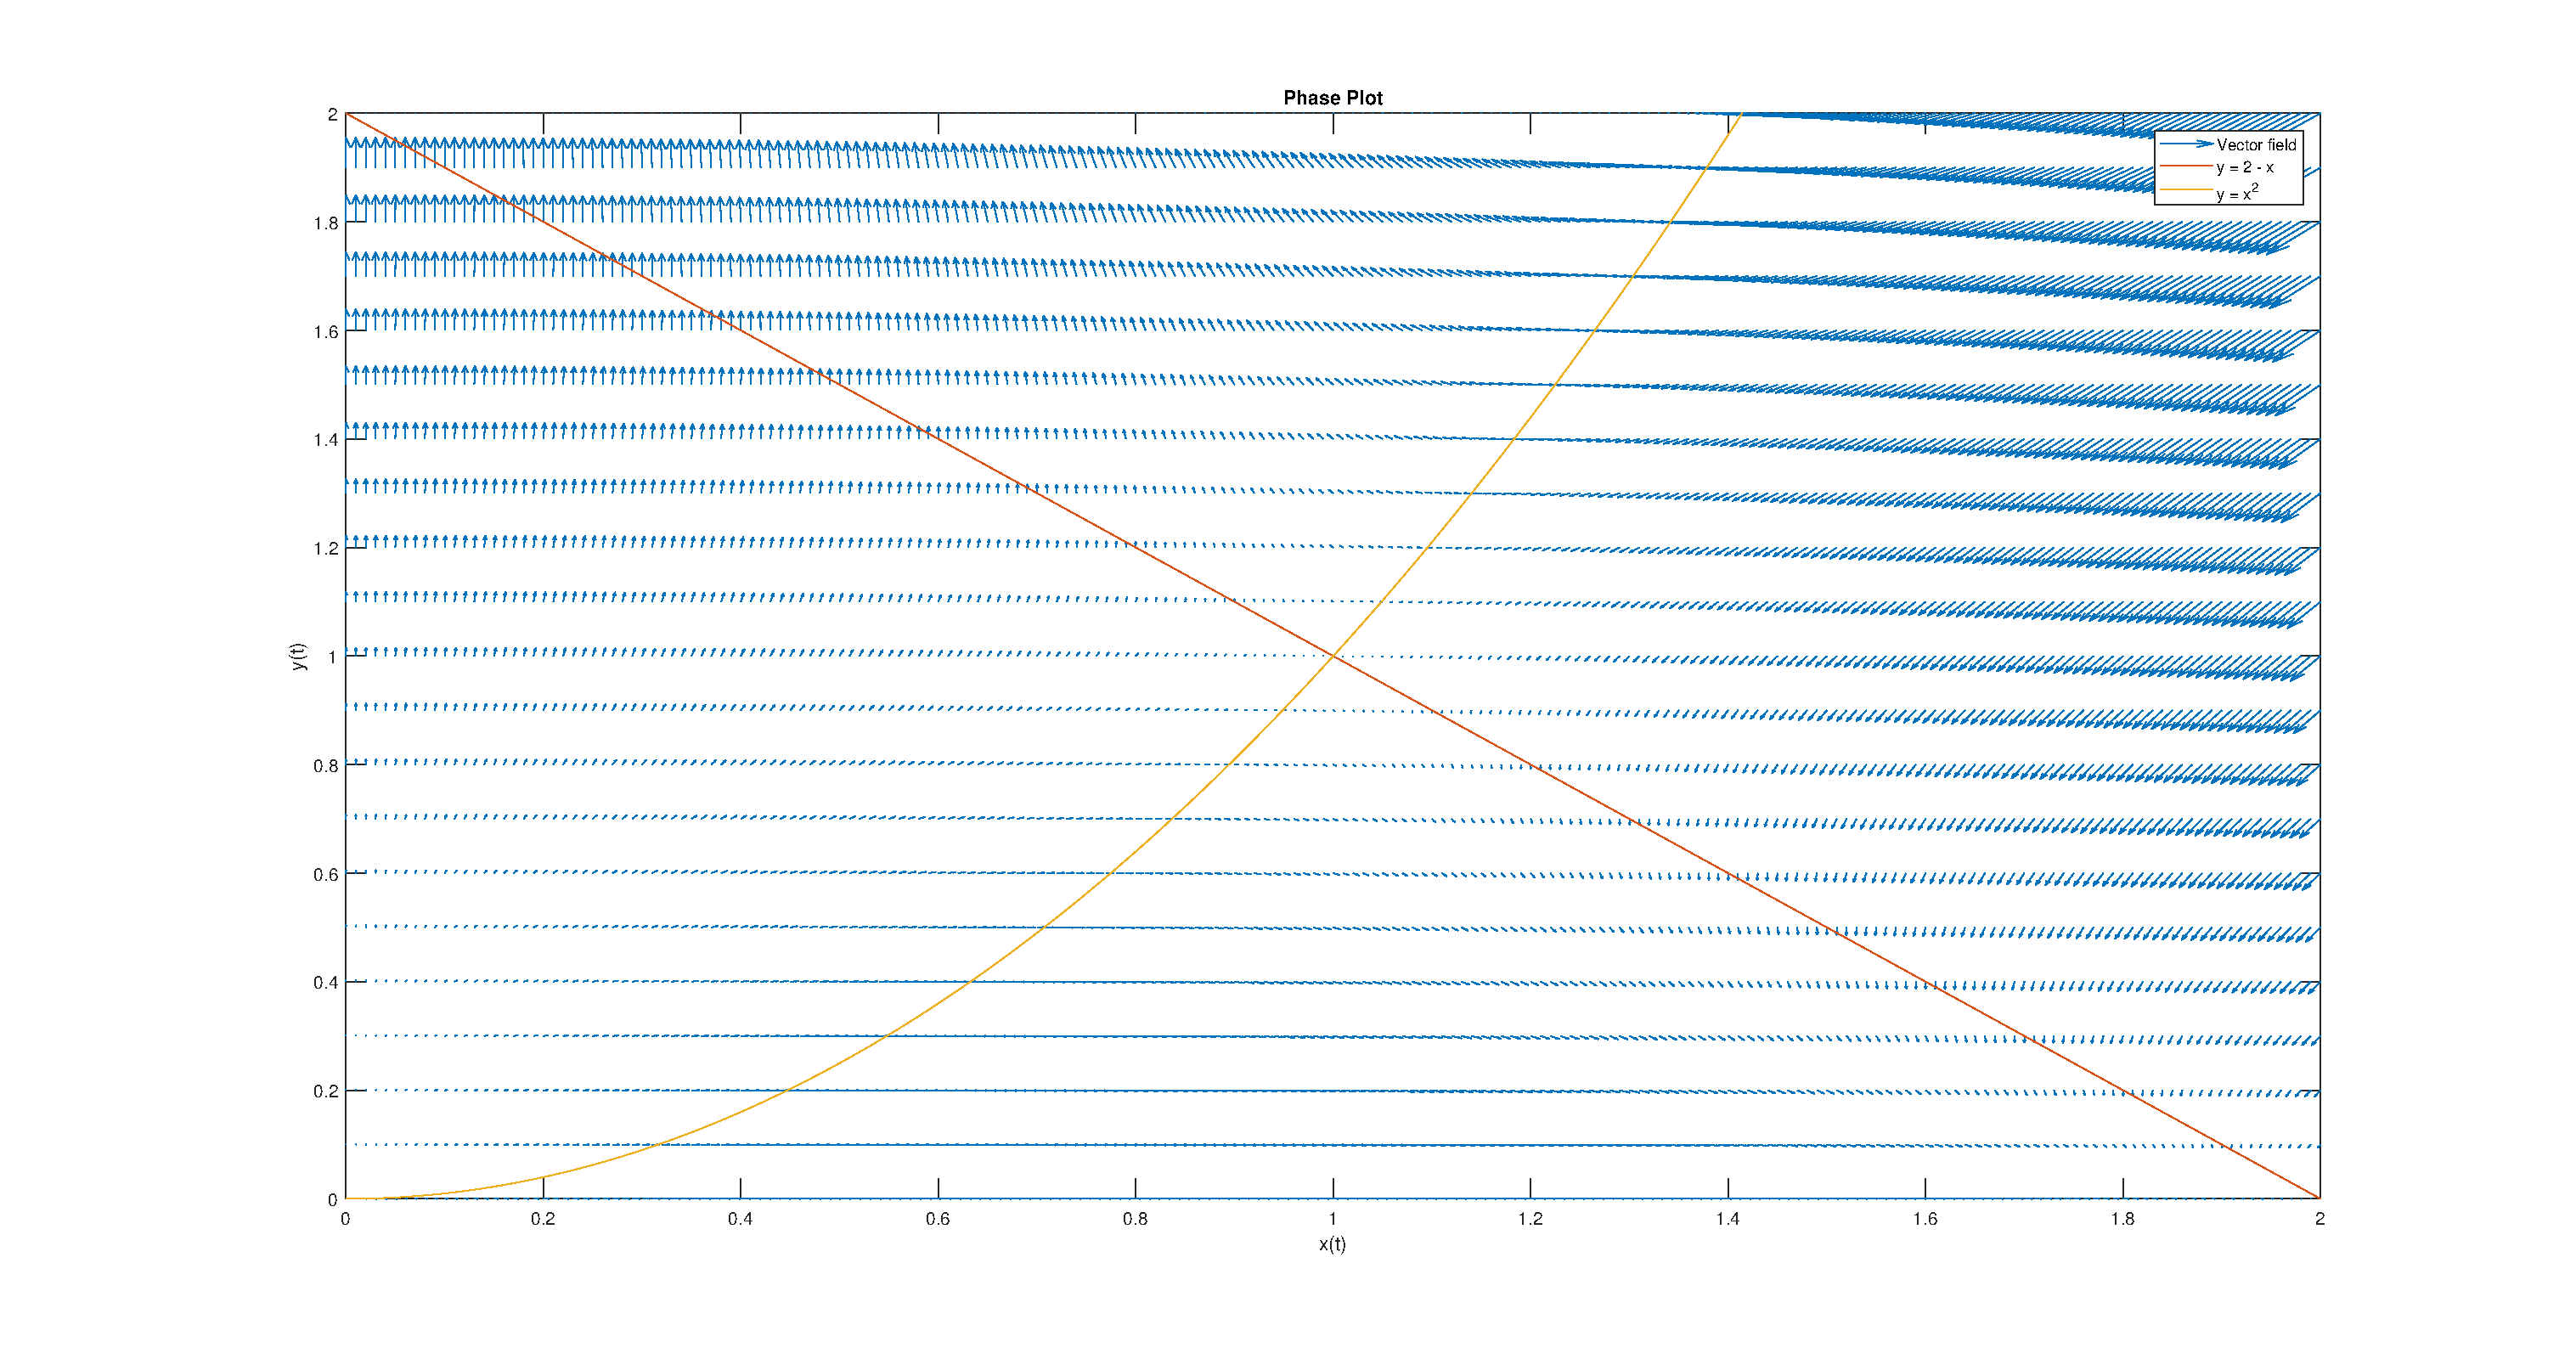
\includegraphics[width=1\linewidth]{Figures/example_2}
	\caption{Nullclines and vector fields}
	\label{fig:example2}
\end{figure}
\end{Example}
\section{Hamiltonian Systems}
\section{Dissipative Systems}

\bibliography{citations}
\bibliographystyle{plain}

\end{document}
